% ----------------------------------------------------------
% Paket och definitioner
\documentclass[11pt, titlepage, oneside, a4paper]{article}	% Dokumentspecifikation
\usepackage[swedish]{babel}									% Språk
\usepackage[T1]{fontenc}									% Teckenkodning för output
\usepackage[utf8]{inputenc}									% Teckenkodning för input
\usepackage{amssymb, graphicx, fancyhdr}					% Symboler och grafik
\usepackage{amsmath}										% Matematiska uttryck
\usepackage{amsthm,algorithm,algorithmic,yhmath,enumitem,lscape} % Algoritmer
\usepackage{float}											% Placeringar av grafik mm.
\usepackage{hyperref, url}									% Webbadresser och referenser
\usepackage{listings}										% Lista källkod
\lstset{
	frame=single,
	title=\lstname,
	numbers=left,
	basicstyle=\tiny
}															% Formatering för listning av källkod

\def\school{Erik Dahlbergsgymnasiet, Jönköping}				% Skolans namn
\def\class{T4}												% FYLL I DIN KLASS
\def\programme{Teknikprogrammet, \class}					% Program
\def\documenttype{Laborationsrapport}						% Typ av dokument
\def\course{Webbutveckling\\ Webbserverprogramering\\Datalagring}	% FYLL I KURS ELLER OMRÅDE
\def\title{Harohal}											% FYLL I UPPG. NAMN
\def\student{Harohal \& co}										% FYLL I DITT NAMN
\def\email{-}												% FYLL I DIN E-POST
\def\graders{Rickard Karlsson}								% FYLL I NAMN PÅ LÄRARE

\setlength{\parindent}{0pt}									% Ta bort indentering
\setlength{\parskip}{10pt}									% Lägg till mellanrum vid nytt stycke

% ----------------------------------------------------------
% Dokumentstart
\begin{document}

% ----------------------------------------------------------
% Framsida
\begin{titlepage}
	\thispagestyle{empty}
	\begin{normalsize}
		\begin{tabular}{@{}p{\textwidth}@{}}
			\textbf{\school \hfill \today} \\
			\textbf{\programme \hfill \documenttype} \\
		\end{tabular}
	\end{normalsize}
	\vspace{25mm}
	\begin{center}
		\huge{\textbf{\course}}\\
		\vspace{10mm}
		\LARGE{\title} \\
		\vspace{15mm}
        \LARGE{version 1.0} \\
        \vspace{10mm}
		\begin{large}
			\begin{tabular}{ll}
				\textbf{Namn} & \student \\
				\textbf{E-post} & \email \\
                
			\end{tabular}
		\end{large}
		\vfill
        \vfill
		\large{\textbf{Bedömning}}\\
		\mbox{\large{\graders}}
	\end{center}
\end{titlepage}
    
% Sidhuvud
\lhead{\footnotesize\student, \today}
\rhead{\nouppercase{\footnotesize\leftmark}}
\pagestyle{fancy}
\renewcommand{\headrulewidth}{0.2pt}

% ----------------------------------------------------------
% Innehållsförteckning.
\pagenumbering{roman}
\tableofcontents

\newpage

% Sidnumrering med arabiska siffror.
\pagenumbering{arabic}
    
% ----------------------------------------------------------
% Dokumentets innehåll    


\newpage

\section{Funktioner}

\begin{tabular}{ll}
\hline
Funktionsnamn & Lägg till Annons                        \\ \hline
Beskrivning   & Lägga till en ny Annons på startsidan \\ \hline
Indata        & namn, beskrivning, länk, bild         \\ \hline
Utdata        & annonsID                              \\ \hline
\end{tabular}

\begin{tabular}{ll}
\hline
Funktionsnamn & Ta bort Annons                        \\ \hline
Beskrivning   & Ta bort en Annons på startsidan \\ \hline
Indata        & annonsID         \\ \hline
Utdata        & Aktiv = falsk                              \\ \hline
\end{tabular}

\begin{tabular}{ll}
\hline
Funktionsnamn & Ändra Annons                       \\ \hline
Beskrivning   & Ändra beskrivning och titel av en annons \\ \hline
Indata        & annonsID, namn, beskrivning, datum, bild, länk   \\ \hline
Utdata        & Lyckad redigering                             \\ \hline
\end{tabular}

\begin{tabular}{ll}
\hline
Funktionsnamn & Skapa konto                     \\ \hline
Beskrivning   & Skapar ett nytt konto \\ \hline
Indata        & Förnamn, efternamn, mail, personnummer, lösenord, telefon   \\ \hline
Utdata        & personID              \\ \hline
\end{tabular}

\begin{tabular}{ll}
\hline
Funktionsnamn & Logga in                     \\ \hline
Beskrivning   & Logga in på webbsidan \\ \hline
Indata        & Lösenord, användarnamn   \\ \hline
Utdata        & personID              \\ \hline
\end{tabular}

\begin{tabular}{ll}
\hline
Funktionsnamn & Byta lösenord                    \\ \hline
Beskrivning   & Byta lösenord på webbsidan \\ \hline
Indata        & Gammalt lösenord, Nytt lösenord   \\ \hline
Utdata        & True/False              \\ \hline
\end{tabular}

\begin{tabular}{ll}
\hline
Funktionsnamn & Verifiera konto                    \\ \hline
Beskrivning   & Verifierar ditt konto från email  \\ \hline
Indata        & GUID   \\ \hline
Utdata        & bekräftatEmail = sant, mail, förnamn, efternamn    \\ \hline
\end{tabular}

\begin{tabular}{ll}
\hline
Funktionsnamn & Ny nyhet                    \\ \hline
Beskrivning   & För att lägga till nyhet \\ \hline
Indata        & nyhetsdatum, nyhetsbeskrivning, publiceradatum, titel \\ \hline
Utdata        & True/false, nyhets ID              \\ \hline
\end{tabular}

\begin{tabular}{ll}
\hline
Funktionsnamn & Ta bort nyhet                   \\ \hline
Beskrivning   & Ta bort en nyhet ifrån sida \\ \hline
Indata        & nyhetsdatum, nyhetsbeskrivning, publiceradatum, titel \\ \hline
Utdata        & Publicerad = falsk            \\ \hline
\end{tabular}

\begin{tabular}{ll}
\hline
Funktionsnamn & Ändra nyhet                   \\ \hline
Beskrivning   & Ändra beskrivning och titel av en nyhet \\ \hline
Indata        & nyhetsdatum, nyhetsbeskrivning, publiceradatum, titel, nyhetsID \\ \hline
Utdata        & True/False            \\ \hline
\end{tabular}

\begin{tabular}{ll}
\hline
Funktionsnamn & Boka                  \\ \hline
Beskrivning   & Bokar en massage med en massör under en viss tid \\ \hline
Indata        & anställdID, tjänstID, startTid, slutTid pris, \\ \hline
Utdata        & True/false, ev.Ny rad på ordrar med unikt orderID, ev.stadie = aktiv            \\ \hline
\end{tabular}

\begin{tabular}{ll}
\hline
Funktionsnamn & Avboka obetald order                  \\ \hline
Beskrivning   & Avbokning för en bokning som är obetald \\ \hline
Indata        & OrderID \\ \hline
Utdata        & True/False, ev.Lyckad borttagning     \\ \hline
\end{tabular}

\begin{tabular}{ll}
\hline
Funktionsnamn & Avboka betald order                  \\ \hline
Beskrivning   & Avbokning för en bokning som är betald \\ \hline
Indata        & OrderID \\ \hline
Utdata        & True/False, ev.Lyckad borttagning, särskild administrativ återbetalning  \\ \hline
\end{tabular}

\begin{tabular}{ll}
\hline
Funktionsnamn & Hämta anställdinfo                  \\ \hline
Beskrivning   & Hämtar information kring en viss anställd \\ \hline
Indata        & anställdID \\ \hline
Utdata        & Namn, beskrivning, bild, behandlarMän/Kvinnor  \\ \hline
\end{tabular}

\begin{tabular}{ll}
\hline
Funktionsnamn & Lägg till anställd                 \\ \hline
Beskrivning   & Lägger till en ny anställd i systemet \\ \hline
Indata        & namn, beskrivning, tjänstID, behandlarMän/Kvinnor, bild \\ \hline
Utdata        & anställdID  \\ \hline
\end{tabular}

\begin{tabular}{ll}
\hline
Funktionsnamn & Ta bort anställd                 \\ \hline
Beskrivning   & Inaktiverar en anställd i systemet \\ \hline
Indata        & anställdID   \\ \hline
Utdata        & Aktiv = falsk  \\ \hline
\end{tabular}

\begin{tabular}{ll}
\hline
Funktionsnamn & Hämta schema                 \\ \hline
Beskrivning   & Hämtar en anställds schema för en specifik vecka \\ \hline
Indata        & anställdID, vecka, år \\ \hline
Utdata        & anställdID, starttid, sluttid, datum  \\ \hline
\end{tabular}

\begin{tabular}{ll}
\hline
Funktionsnamn & Ta bort schema                 \\ \hline
Beskrivning   & Tar bort en anställdstid för ett pass \\ \hline
Indata        & anställdID, starttid, vecka, år \\ \hline
Utdata        & True/False, ev lyckad borttagning  \\ \hline
\end{tabular}

\begin{tabular}{ll}
\hline
Funktionsnamn & Kopira schematid                 \\ \hline
Beskrivning   & Kopierar schema ifrån en annan veckas schema \\ \hline
Indata        & Sluttider, starttider, vecka, nyvecka \\ \hline
Utdata        & True/False, ev nytt schema  \\ \hline
\end{tabular}

\begin{tabular}{ll}
\hline
Funktionsnamn & Ny tjänst              \\ \hline
Beskrivning   & Lägger till en ny tjänst i systemet \\ \hline
Indata        & namn, beskrivning, tid, pris, bild \\ \hline
Utdata        & tjänstID  \\ \hline
\end{tabular}

\begin{tabular}{ll}
\hline
Funktionsnamn & Ta bort tjänst              \\ \hline
Beskrivning   & Flagga tjänst som inaktiv \\ \hline
Indata        & tjänstID  \\ \hline
Utdata        & Aktiv = falsk  \\ \hline
\end{tabular}

\begin{tabular}{ll}
\hline
Funktionsnamn & Ändra tjänst              \\ \hline
Beskrivning   & Ändrar informationen om tjänst \\ \hline
Indata        & tjänstID, namn, beskrivning, bild, pris, tid,   \\ \hline
Utdata        & True/False, Lyckad ändring  \\ \hline
\end{tabular}


\newpage

\section{Scenarier}
\textbf {En person besöker hemsidan }

När personen besöker sidan på nytt så ska den komma till en Välkommen sida. På denna sida så står det nyheter och man blir introducerad till navigationsfunktionen.  Det finns inget naturligt element i navigationen som dirigerar användaren till denna sida igen och användaren får själv välja vad den vill besöka näst.

\textbf {En person loggar in}

En person navigerar från valfri sida till navigationselementet ”Logga in”. En person som redan har ett konto kan ange sina uppgifter för att sedan logga in och bli dirigerad till landningssidan, uppgifterna måste givetvis vara stämma överens med de som den uppgav när den registrerade sig. Valet att registrera sig finns som en knapp. Det finns även ett val att återställa sitt lösenord, även detta val kommer med en knapp. När man klickar på knappen så kommer blir man dirigerad till en sida där man får skriv in sin mail. Detta skickar ett mail till personens konto med en länk som återställer lösenordet och den får välja ett nytt lösenord.

\textbf {En Person registrerar sig}

En person går in på hemsidan för första gången i sitt liv. Han klickar på “skapa konto”. Han kommer till en skärm där han får fylla i kontaktuppgifter och lösenord. Han får sedan ett mail där han får bekräfta sitt konto.

\textbf {En Person beställer tid}

Personen fortsätter sedan sin resa efter att skapat kontot(se ovan) och klickar sig in på boka tid fliken. Där ser han ett tidsschema över de lediga tiderna och väljer själv när det passar honom utefter de lediga tiderna som visas. Han väljer också vilken typ av massage han vill ha och bekräftar sedan bokningen.

\textbf {En Person beställer flera tider}

En person har nu bokat en tid för en massage, men önskar boka en ytterligare massage. Efter att personen fyllt i en bokning och tryckt på “boka”-knappen läggs personens bokning till i en lista av bokningar, och personen kan helt enkelt upprepa bokningsprocessen tills personen är nöjd, och kan sedan klicka på slutför och gå vidare till bekräftelsesidan för eventuell betalning.

\newpage
\textbf {En person vill avboka sin tid}

Om en person av någon anledning önskar ta bort sin bokade tid klickar personen sig vidare till ”Min profil. Där finns en lista för alla personens kommande bokningar, och för varje bokad tid kan personen markera bokningen med ”markera”-checkrutan, sedan trycka på knappen ”Avboka markerade”. Då kommer en pop-up ruta som frågar om du önskar avboka valda bokningar. Trycker personen ”Ja” kommer bokningen tas bort. Vill personen avboka ett flertal bokningar trycker personen in alla bokningar hen önskar ta bort, och trycker på ”Avboka markerade”, då kommer en pop-up som frågar om du önskar ta bort följande bokningar, och om hen konfirmerar sitt val kommer bokningarna tas bort

\textbf {En person vill ändra sina kontoinställningar}

Personen går in på sina kontosida/mina sidor/profil. någonstans på sidan så finns det ett kugghjul där man kan ändra kontoinställningar, exempelvis ändra mail, lösenord, adress och nummer.

\textbf {En person tar bort sitt konto }

Om en person önskar ta bort sitt konto klickar sig personen till sidan “Din profil”, där det längst ner på sidan finns en knapp “Ta bort detta konto”. Efter att klickat på knappen så måste personen bekräfta med lösenord, och efter det är gjort det så skickas ett bekräftelse mail och i den finns en länk som faktiskt tar bort kontot. I databasen tas kontot egentligen inte bort, utan kundnummer etc. sparas för att man ska kunna bokföra och hålla koll på gamla bokningar.


\newpage

\section{Krav}
\subsection{Konto}
	\subsubsection*{Registrering}
	\begin{itemize}
		\item Det ska finnas fält som ska kunna ta information som input.
		\item Informationen ska anges av den blivande användaren.
		\item Vissa fält får inte lämnas oidentifierade.
		\item Denna information ska sedan.
		\item Efter att informationen är angiven så skickas ett bekräftelsemail.
		\item Försöker en användare logga in utan att ha bekräfta får användaren ett meddelande på skärmen som säger att användaren måste bekräfta sitt konto, samt en knapp för att skicka ett nytt 	bekräftelsemail.
	\end{itemize}
	\subsubsection*{Logga in}
	\begin{itemize}
		\item Det som krävs för inloggning är användarnamn och lösenord. Dessa skall vara angivna och måste vara korrekt. 
		\item Om de är korrekt så skall man föras vidare till landningssidan.
		\item Annars så kommer ett felmeddelande upp och man får försöka igen.
		\item Antalet försök är obestämt.
		\item Alternativet ”Glömt lösenord?” ska finnas och användaren ska då bli dirigerad till en sida där den får ange mail. 
		\item Det kommer i sin tur leda till att man får en länk på sin mail som dirigerar användaren till ännu en sida där användaren får ange sitt nya lösenord två gånger(måste stämma överens).
		\item Användaren blir sedan dirigerad till ”Logga in” och måste ange sina nya uppgifter för att logga in.
	\end{itemize} 

\newpage
	\subsubsection*{Byta lösenord}
	\begin{itemize}
		\item Två fält som båda tar lösenord som input
		\item Lösenorden måste stämma överens, annars felmeddelande
		\item Stämmer allt skickas ett mail till din mail
		\item Mailet innehåller en GUID som låter dig välja ett nytt lösenord
	\end{itemize} 

	\subsubsection*{Glömt lösenord}
	\begin{itemize}
		\item Ett fält som tar din mail som input
		\item Stämmer allt skickas ett mail till din mail
		\item Mailet innehåller en GUID som låter dig välja ett nytt lösenord
	\end{itemize} 

\subsection{Landningssida}
	\begin{itemize}
		\item På landningssidan ska det finnas nyheter och annonser.
		\item Nyheter presenteras i form av sektioner och varje sektion täcker cirka 2/3 av sidans bredd.
		\item Annonserna presenteras också i sektioner och varje sektion täcker den resterade 1/3 av sidans bredd.
		\item Sektionernas höjdjusteras efter innehållets storlek.
	\end{itemize} 

\subsection{Navigation}
	\begin{itemize}
		\item Det finns ett navigeringsfält som har länkar till varje sida som finns nedan. 
		\item Detta kommer att vara statiskt på hemsidan och kommer alltid finnas tillgängligt.
	\end{itemize} 


\newpage
\subsection{Massörer}
	\subsubsection*{Massörer: Användare}
	\begin{itemize}
		\item Ska innehålla informationen om de olika anställda i form av sektioner.
		\item Sektionerna kommer vara sig lika i aspekter och bredd och täcka cirka 2/3 av sidans bredd, men kan komma att variera i höjd beroende på innehållets storlek.
		\item Man ska ha möjligheten att checka en sektion.
		\item Det finns en knappt som heter "Till boka", och de checkade massörerna följer med till bokasidan. 
		\item Det ska finnas en info box som kommer att finnas till höger om alla sektioner. Denna box ska vara statisk och innehålla generell information om massörerna, vilka krav som förväntas m.m. 
	\end{itemize}
	
	\subsubsection*{Massörer: Admin}
	\begin{itemize}
		\item Edit box sektioner.
		\item Edit box box.
		\item Ska kunna redigera innehåll i element och box.
		\item Ska kunna redigera tider.
	\end{itemize} 

\subsection{Tjänster}
	\subsubsection*{Tjänster: Användare}
	\begin{itemize}
		\item Kommer att ha samma upplägg som ”Massörer” fast annorlunda innehåll.
		\item Där fokuseras det mer på vilken massör som utför tjänsten, tider och priser. 
		\item Man kan även checka för en tjänst som sedan kommer att följa med till ”boka”. 
	\end{itemize}
	
	\subsubsection*{Tjänster: Admin}
	\begin{itemize}
		\item Edit box sektioner.
		\item Edit checkbox box.
		\item Kunna redigera innehåll och element.
	\end{itemize}

\subsection{Om oss}
	\subsubsection*{Om Oss: Användare}
	\begin{itemize}
		\item Finnas info om oss.
		\item Hur man kontaktar oss.
		\item Vägbeskrivning (Google maps).
	\end{itemize} 
	
	\subsubsection*{Om oss: Admin}
	\begin{itemize}
		\item Redigera information.
		\item Redigera kontakt info.
		\item Redigera/uppdatera vägbeskrivning.
	\end{itemize}

\subsection{Min profil}
	\subsubsection*{Min Profil: Användare}
	\begin{itemize}
		\item Informationsbox.
		\item Kontaktinformation.
		\item Redigera kontaktinformation.
		\item Lagra och visa genomförda beställningar.
		\item Visa kommande beställningar.
		\item Kunna avboka kommande beställningar.
		\item Knapp för att byta lösenord som omdirigerar dig till byta lösenordssidan
	\end{itemize} 
	\subsubsection*{Min profil: Admin}
	\begin{itemize}
		\item Näst intill identisk till Min Profil.
		\item Tids och datumbaserat schema.
		\item Tillgång till alla anställdas scheman.
		\item kunna redigera scheman.
	\end{itemize}
	\subsubsection*{Min profil: Anställd}
	\begin{itemize}
		\item Näst intill identisk till Min Profil.
		\item Tids och datumbaserat schema.
	\end{itemize}
	
\subsection{Bokningar}
	\subsubsection*{Bokningar: Användare}
	\begin{itemize}
		\item Kunna boka en beställning med valfri tid, massör och tjänst.
		\item Kunna boka flera tider i samma veva.
		\item Kunna betala direkt på hemsidan, på plats eller via räkning.
	\end{itemize}
	\subsubsection*{Bokningar: Admin}
	\begin{itemize}
		\item Kunna visa alla kommande bokningar för alla kunder och massörer.
		\item Ändra och ta bort bokningar.
	\end{itemize}
	
\subsection{Generellt}
\begin{itemize}
	\item Landningssidan ska vara det som visas när man besöker hemsidan.
	\item Snygg, bekväm och lugn design.
	\item Responsiv.
	\item Justeras utefter användarplattform(pc, smartphone, padda etc.)
\end{itemize}

\newpage
\section{Databasdiagram}
\begin{center}
	\textit{Diagram över vår databas}
    \includegraphics[width=1\textwidth]{../Bilder/databasdiagram.png}
\end{center}
\newpage

\section{Wireframe}
Detta är våra wireframe bilder. Här finns vanliga versioner och admin versioner. Den större skillnaden mellan admin sidorna och de vanliga sidorna är att admins kan ändra det mesta på alla sidor samt att de inte har någon boknings knapp utan de kan istället gå in och kolla på alla bokningar. Admins har också scheman på deras profil så de ser dem. Vi kommer behöva 2 ”nivåer” av admins. Den lägre nivån kommer inte kunna redigare mer än sin beskrivning på Massörer-sidan och de kommer se sitt schema på sin profil. Den högre nivån vilket kommer troligtvis vara ägaren kommer kunna redigera allt. På ägarens profil har den också så att den kan sätta alla arbetares schema, detta är dock inte visat i bilderna nedan.
\newpage
\begin{center}  	
  	\textit{Landningssida}
    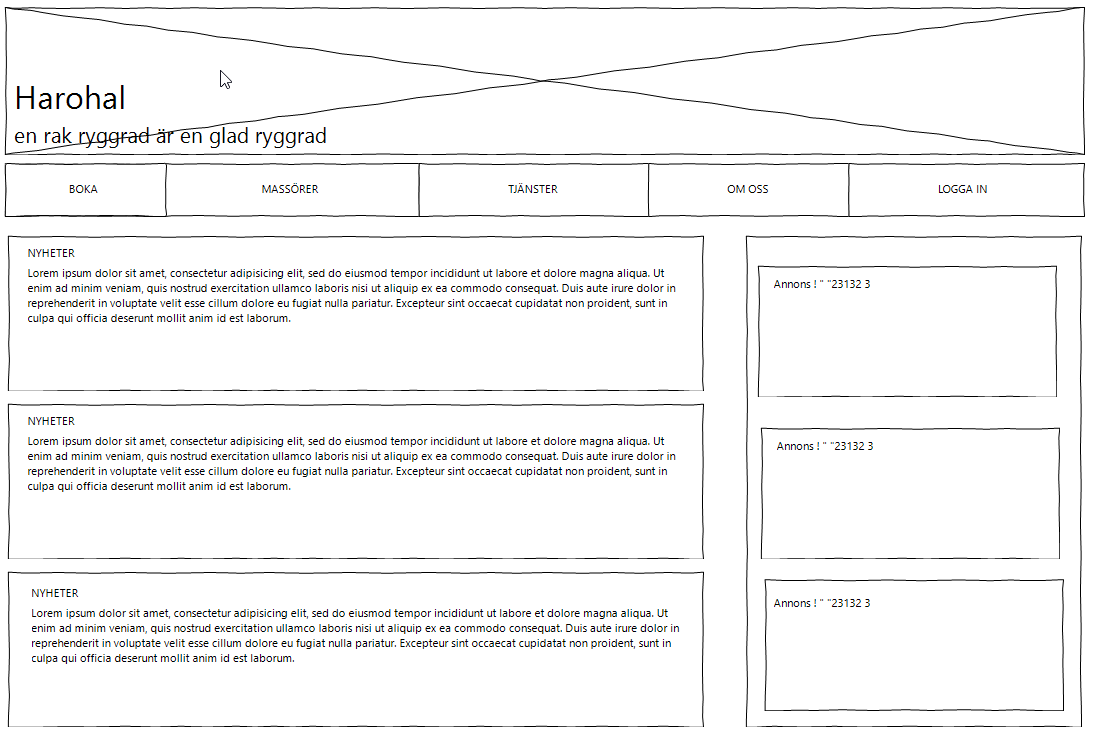
\includegraphics[width=1\textwidth]{../Bilder/Wireframe/hem}
    
    \textit{Logga in}
    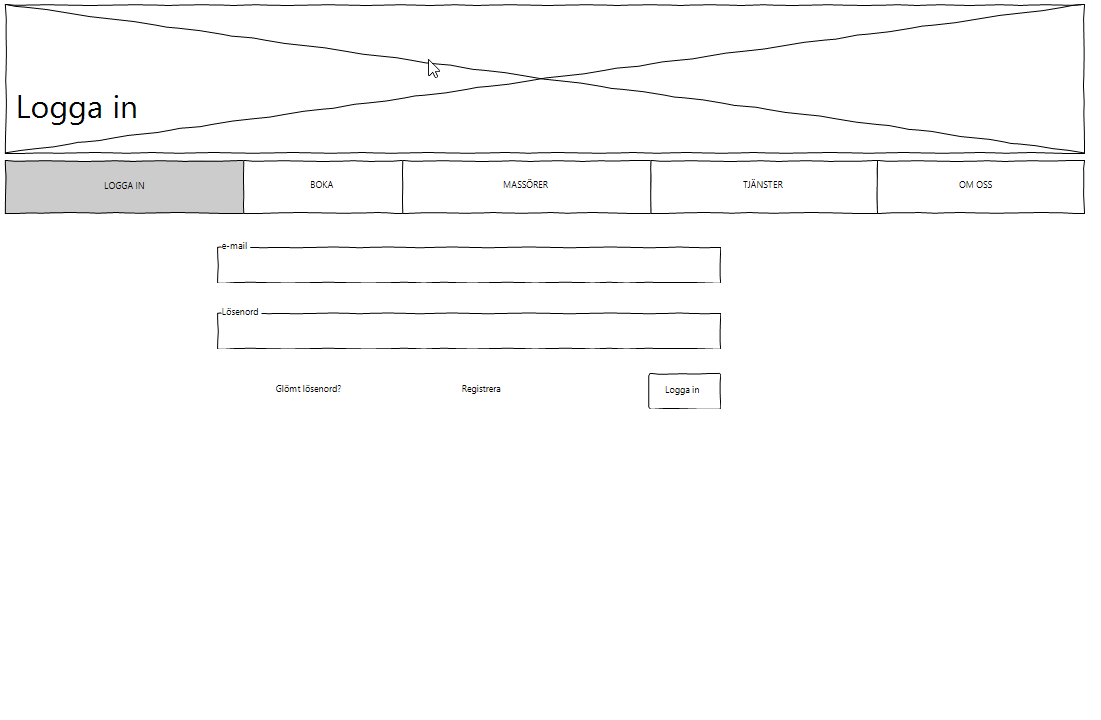
\includegraphics[width=1\textwidth]{../Bilder/Wireframe/logga_in}
    \newpage
    
    \textit{Registrera ny användare}
    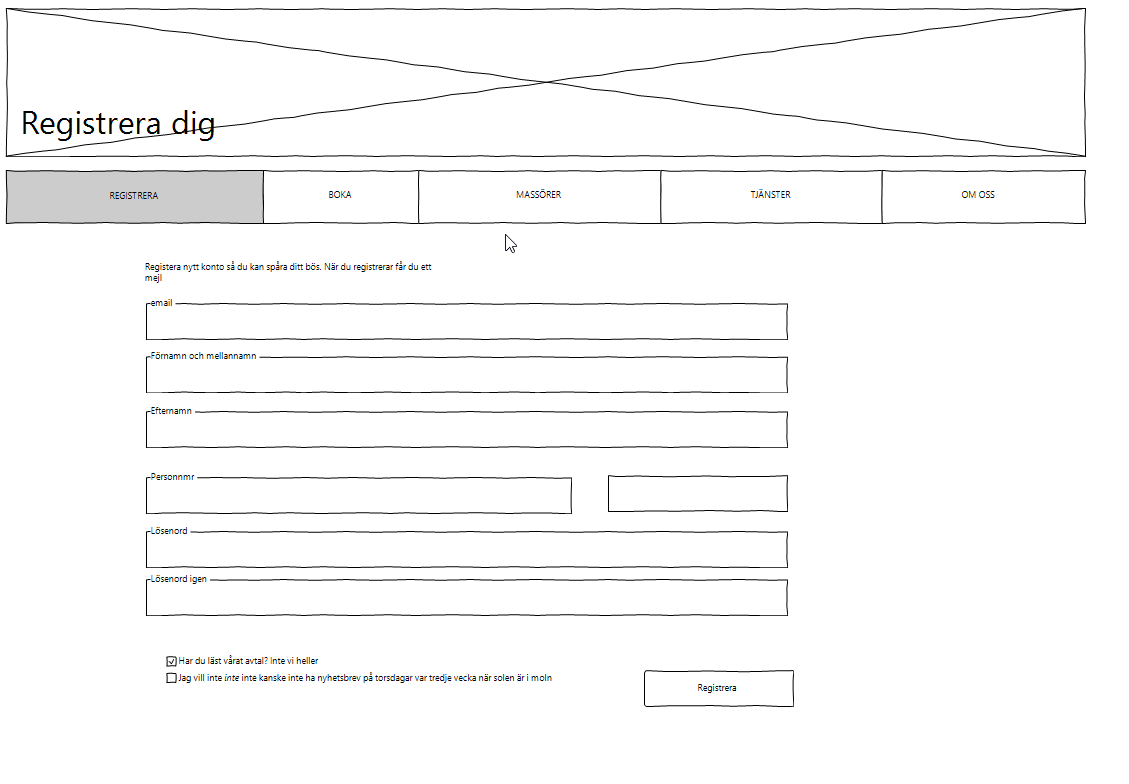
\includegraphics[width=1\textwidth]{../Bilder/Wireframe/registrera}
    
    \textit{Glömt ditt lösenord}
    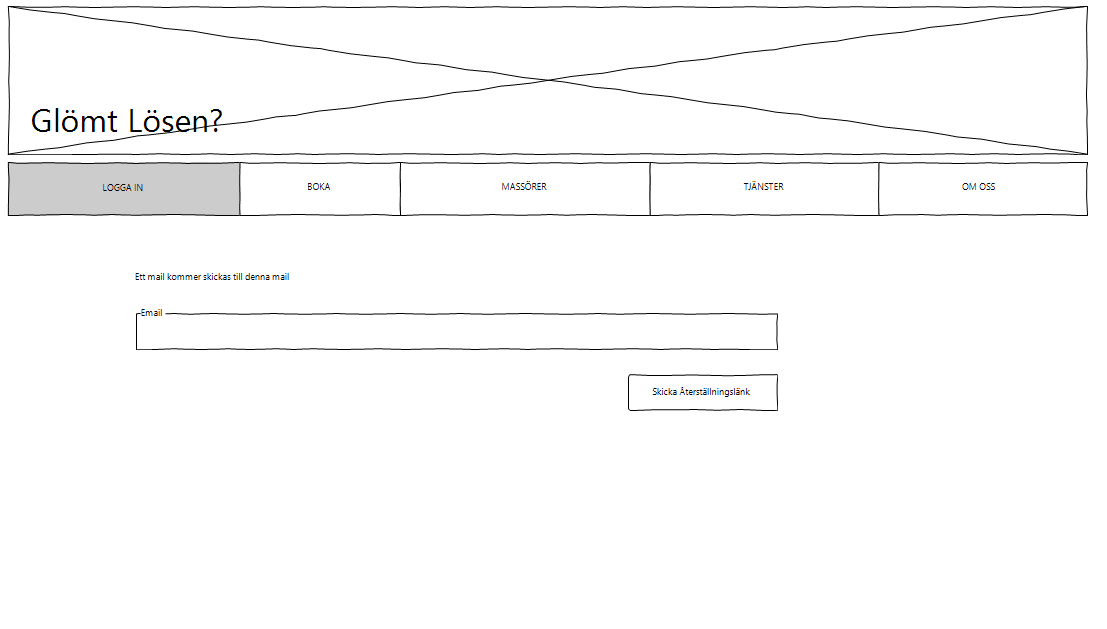
\includegraphics[width=1\textwidth]{../Bilder/Wireframe/glomt_losen}
    \newpage
    
    \textit{Återställ lösenord}
    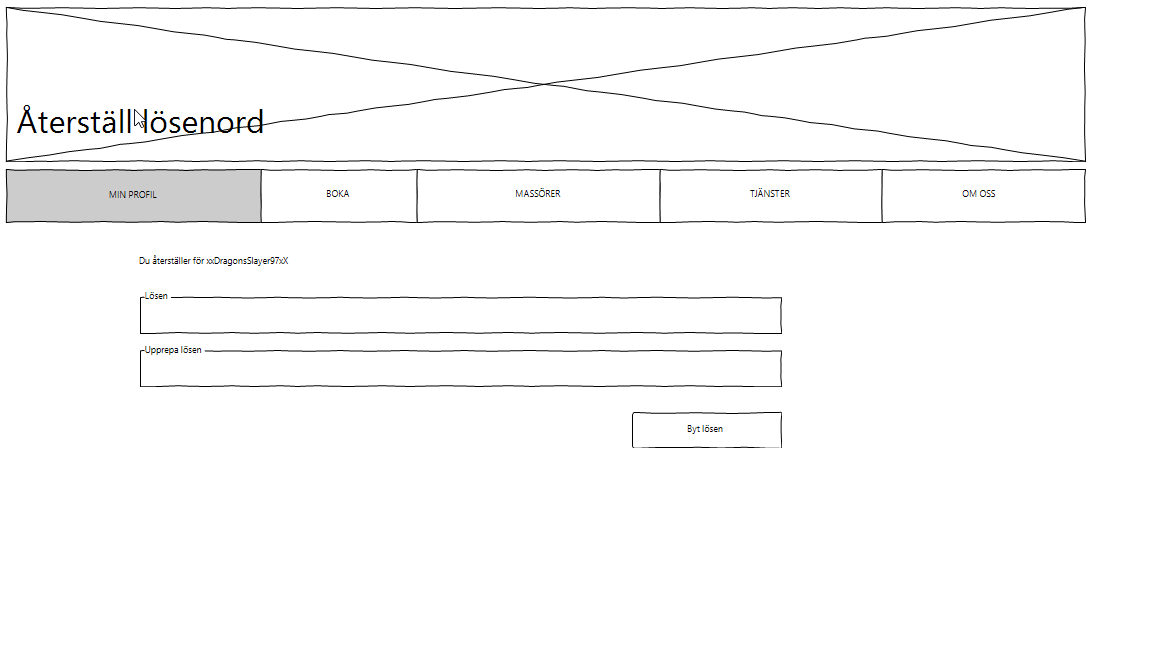
\includegraphics[width=1\textwidth]{../Bilder/Wireframe/aterstall_losenord}
    
    \textit{Min profil}
    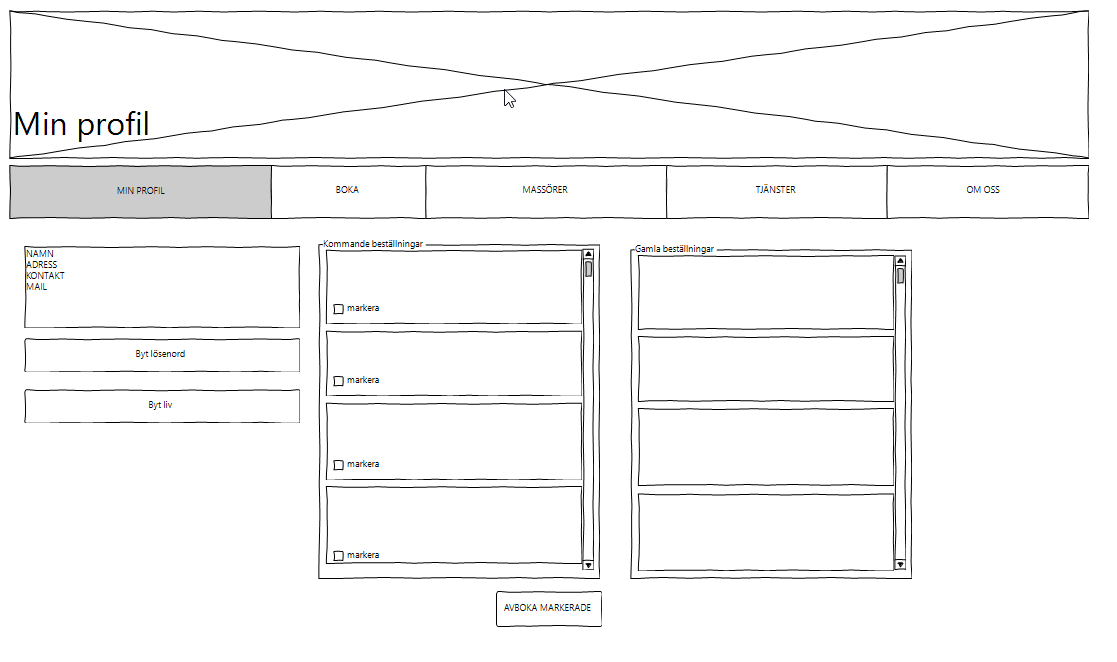
\includegraphics[width=1\textwidth]{../Bilder/Wireframe/min_profil}
    \newpage
    
    \textit{Boka}
    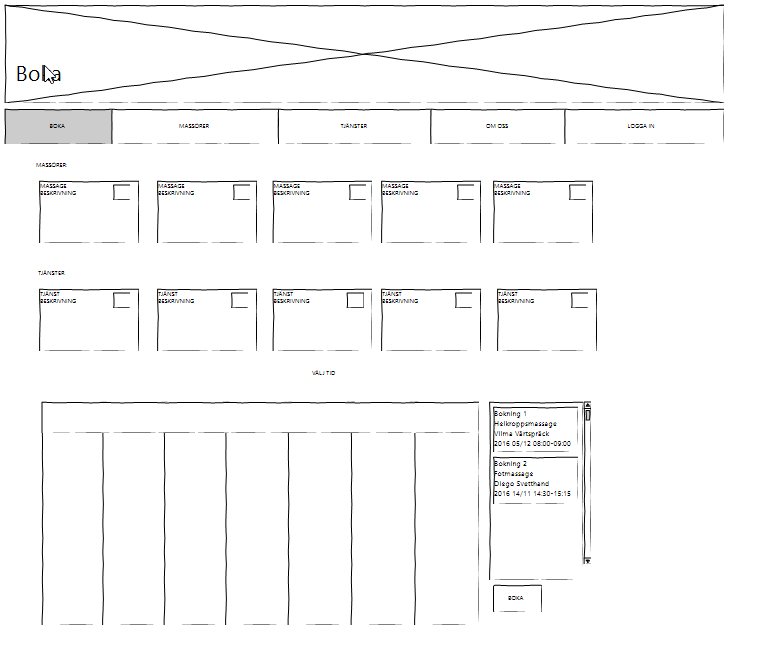
\includegraphics[width=1\textwidth]{../Bilder/Wireframe/boka}
    
    \textit{Bekräfta bokning}
    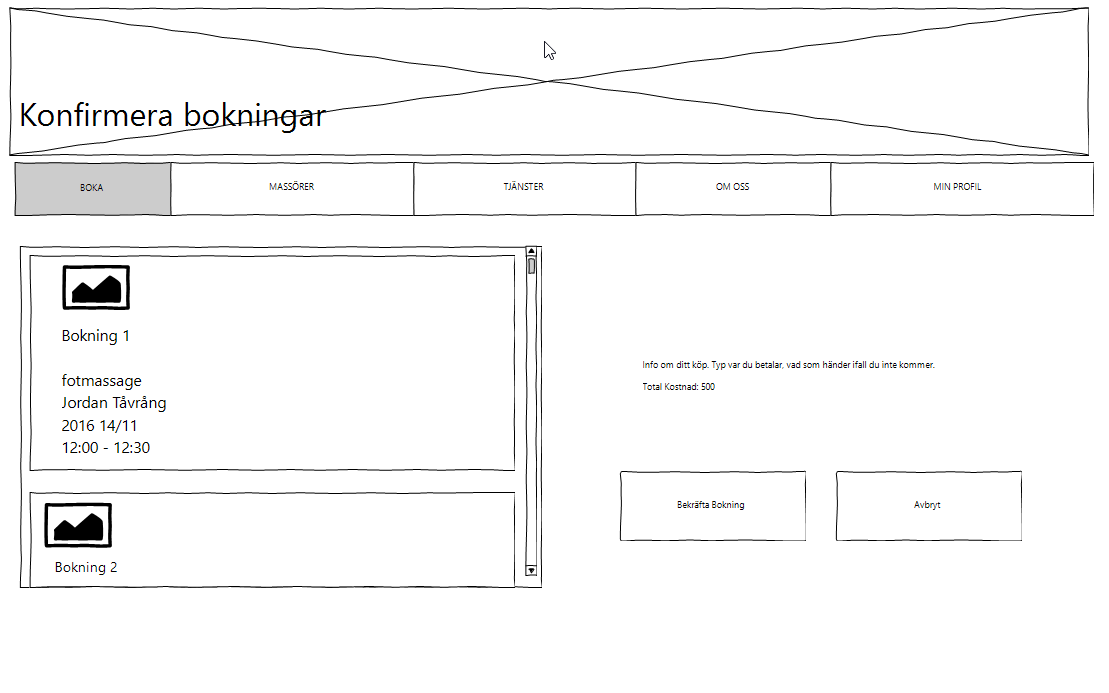
\includegraphics[width=1\textwidth]{../Bilder/Wireframe/bekrafta_bokning}
    \newpage
    
    \textit{Massörer}
    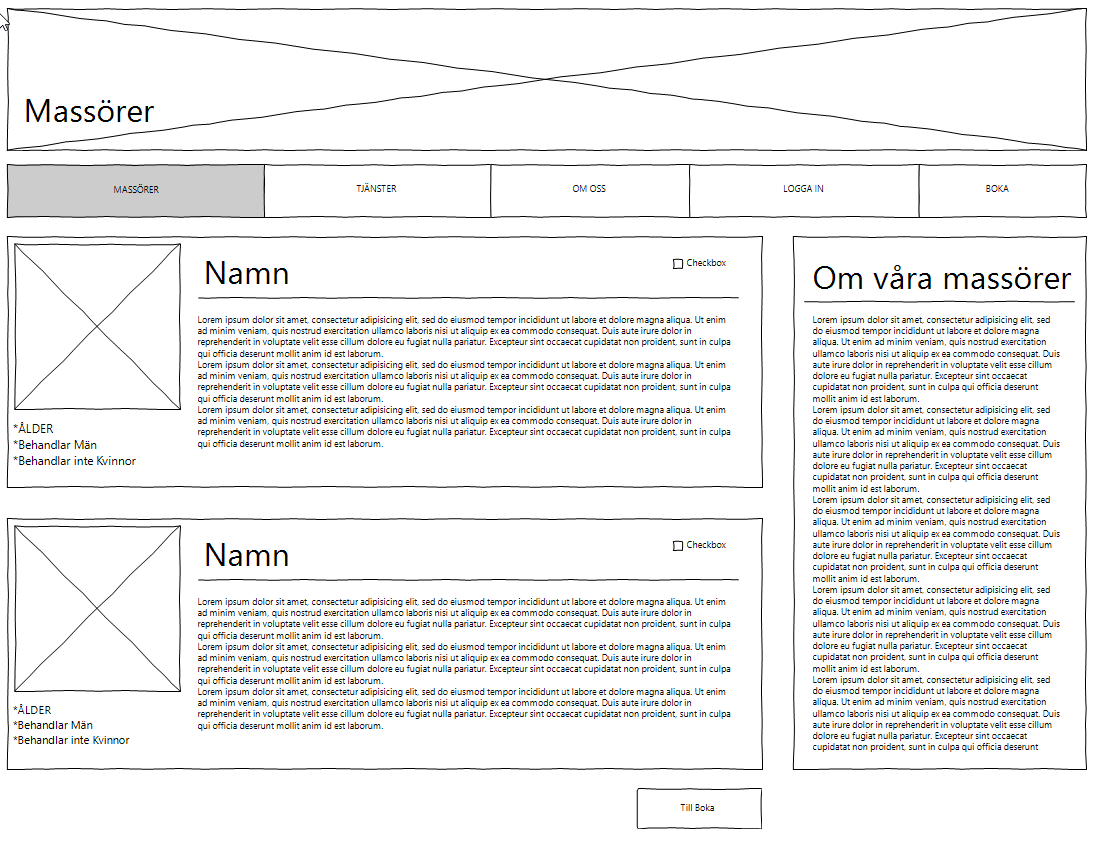
\includegraphics[width=0.9\textwidth]{../Bilder/Wireframe/massorer}
    
    \textit{Tjänster}
    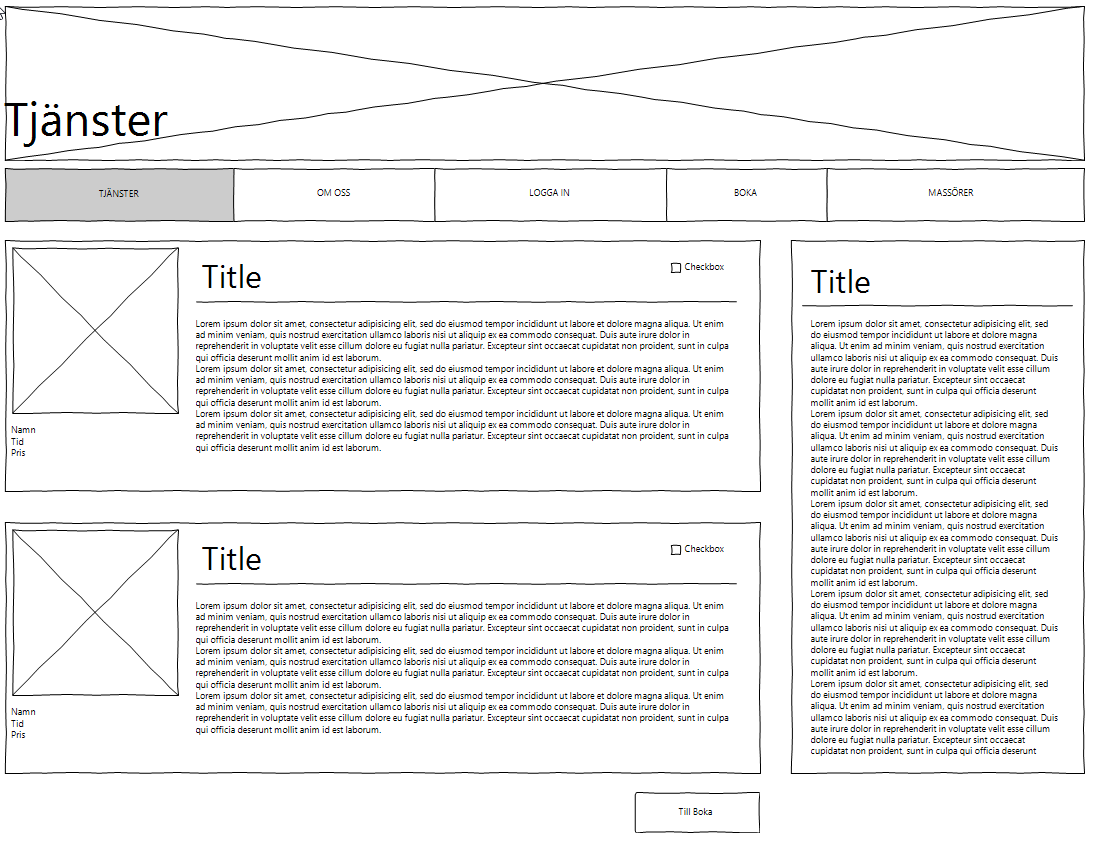
\includegraphics[width=1\textwidth]{../Bilder/Wireframe/tjanster}
    \newpage
    
    \textit{Om oss}
    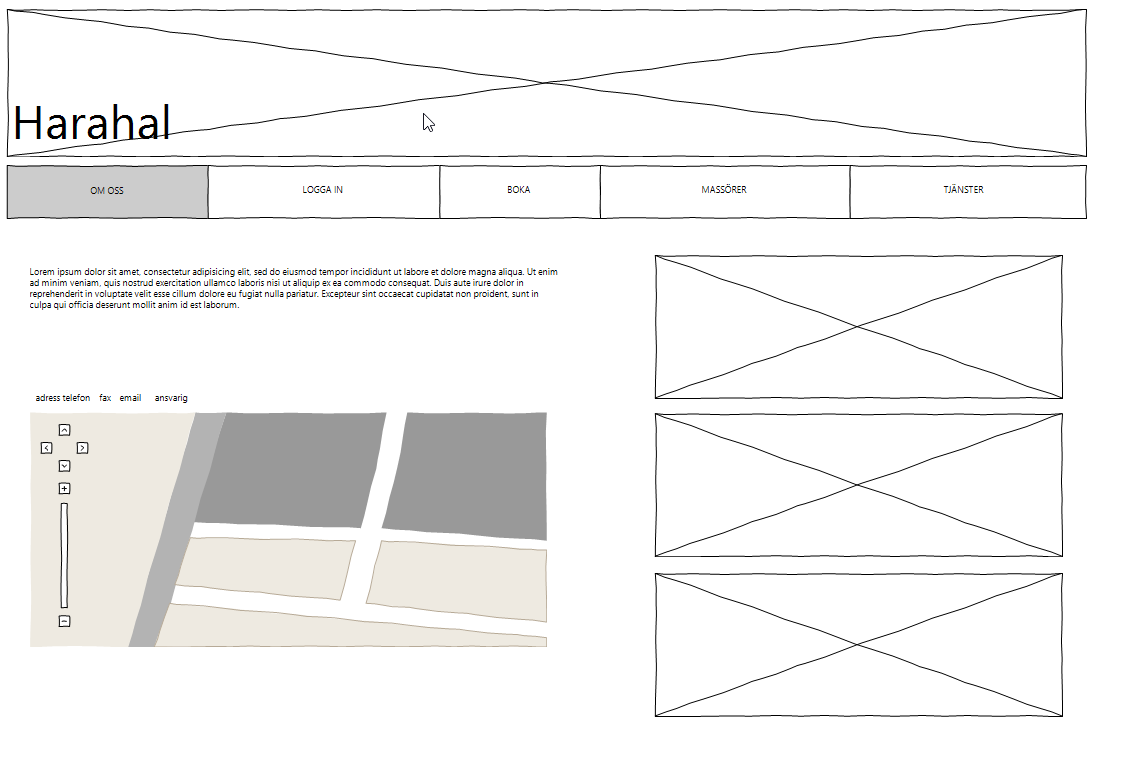
\includegraphics[width=1\textwidth]{../Bilder/Wireframe/om_oss}
    
    \textit{Landningssida för admins}
    \includegraphics[width=1\textwidth]{../Bilder/Wireframe/a_hem}
    \newpage
    
    \textit{Massörer för admins}
    \includegraphics[width=1\textwidth]{../Bilder/Wireframe/a_massorer}
    
    \textit{Tjänster för admins}
    \includegraphics[width=1\textwidth]{../Bilder/Wireframe/a_tjanster}
    \newpage
    
    \textit{Om oss för admins}
    \includegraphics[width=1\textwidth]{../Bilder/Wireframe/a_om_oss}
    
    \textit{Bokningar för admins}
    \includegraphics[width=1\textwidth]{../Bilder/Wireframe/a_bokningar}
    
    
\end{center}


\newpage

\bibliography{references} 
\bibliographystyle{unsrt}
\addcontentsline{toc}{section}{Referenser}

\newpage
\appendix

\end{document}
